\appendix{{\bf QR} Decompositions Using Householder Transformations}
\chaptermark{Householder Transformations}
\label{pcb:qr}

To compute the $QR$ decomposition of an $N \times P$ matrix
$\bX$, we use Householder transformations \cite{hous:1958},
a generalization of reflections in the plane.
These are $N \times N$ matrices of the form
$$
\bH_{{\bu}} = \bI - 2 \bu \bu \trans
$$
where $\bI$ is the $N \times N$ identity matrix and $\bu$ is an
$N$-dimensional unit vector
(that is, $\norm \bu \norm  = \sqrt {\bu \trans \bu} = 1$).
$ \bH_{\bu}$ is symmetric and orthogonal, since
$$
\bH_{\bu} \trans =
\bI \trans -  2 \bu \bu \trans = \bH_{\bu}
$$
and
$$
\bH_{\bu} \trans \bH_{\bu} = \bI - 4 \bu \bu \trans +
4 \bu \bu \trans \bu \bu \trans = \bI
$$

Multiplying a vector $\by$ by $\bH_{\bu}$, as
$$
\bH_{\bu} \by =
\by - 2 \bu \bu \trans \by
$$
corresponds to reflecting $\by$ about the line through the origin
perpendicular to $\bu$, as shown in
Figure~\ref{fig:Householder}.
\begin{figure}
  \centerline{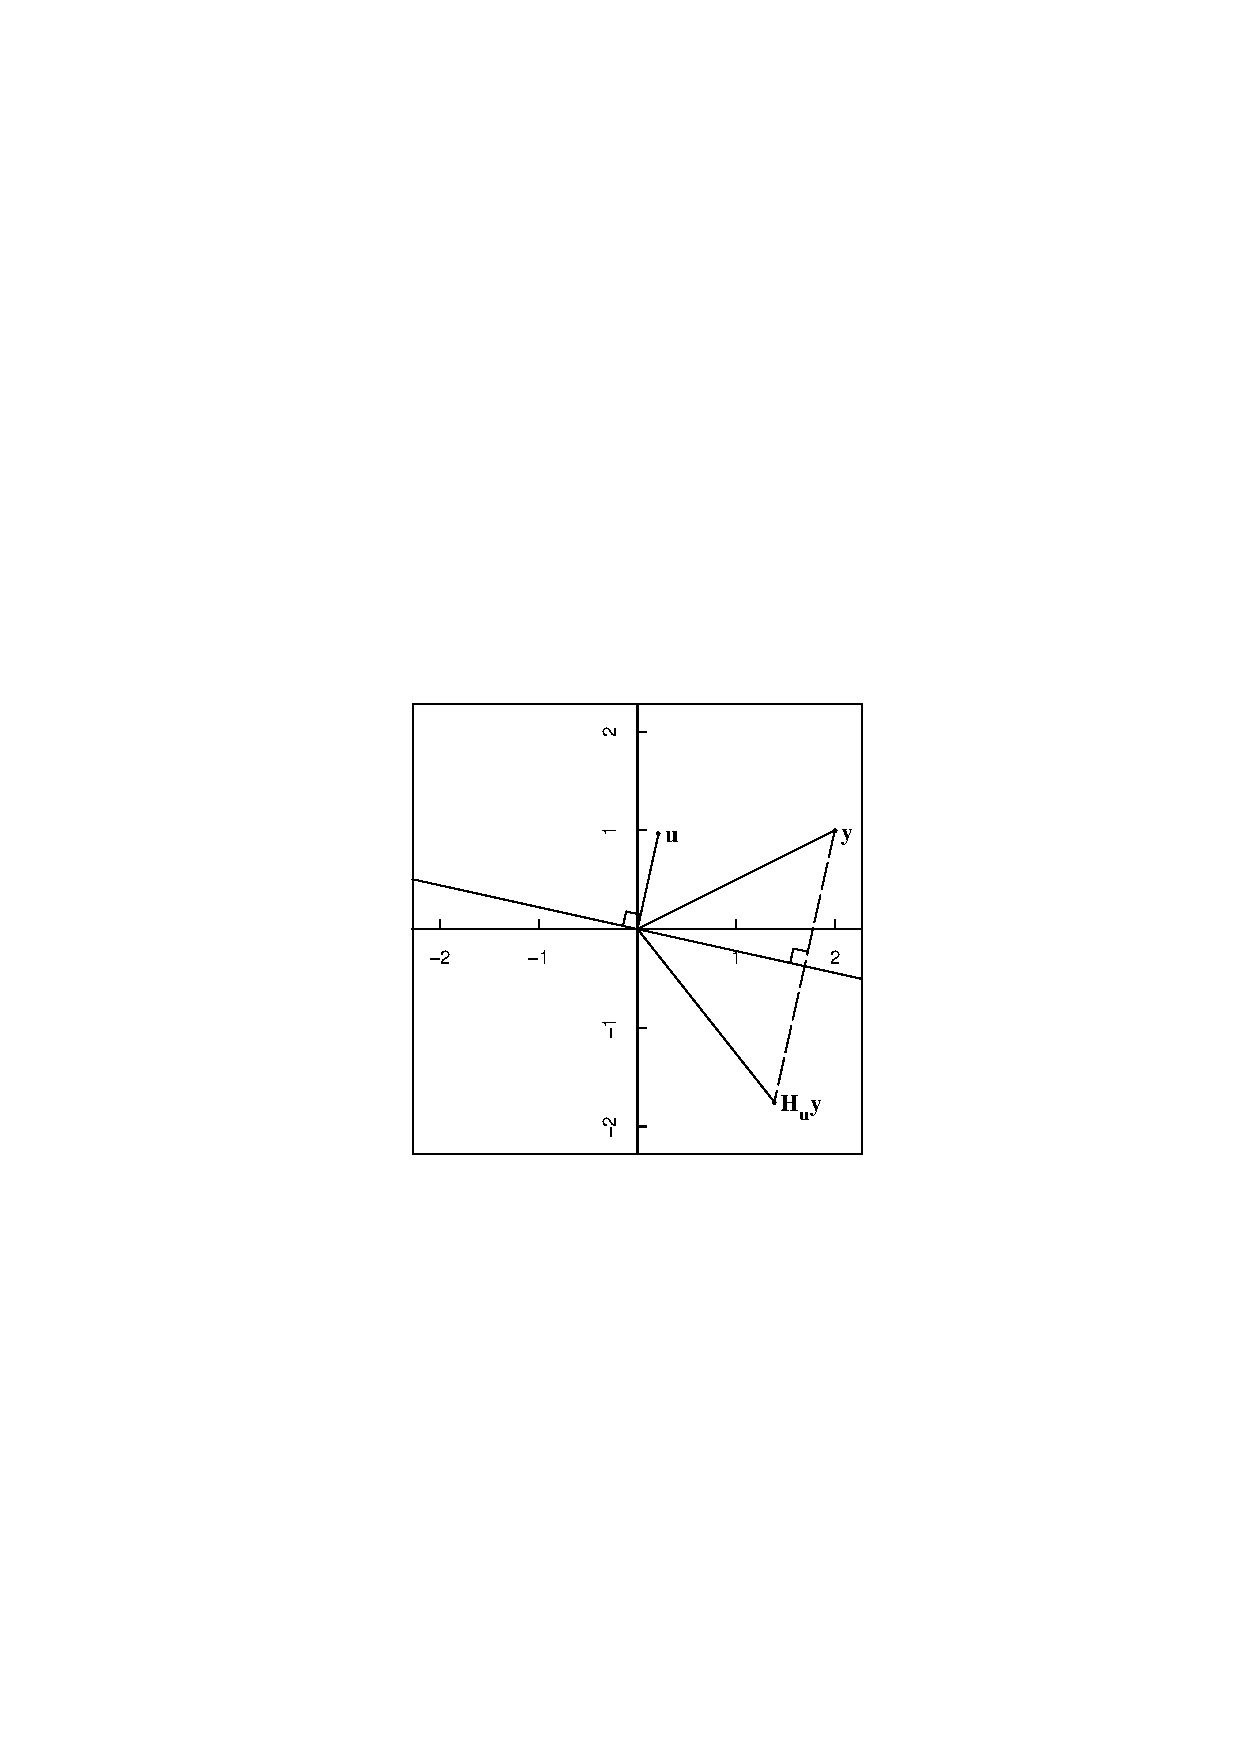
\includegraphics{A2Householder}}%,height=2.25in}}
  \caption{\label{fig:Householder}
  A Householder transformation showing the reflection about the line
  perpendicular to $\bu$ of the vector $\by$ to form $\bH_{\bu} \by$.}
\end{figure}
By choosing
\begin{equation}
  \bu={\by-\norm\by\norm\be_1\over\norm(\by-\norm\by\norm\be_1)\norm}
  \label{eqn:1.16a}
\end{equation}
or
\begin{equation}
  \bu={\by+\norm\by\norm\be_1\over\norm(\by+\norm\by\norm\be_1)\norm}
  \label{eqn:1.16b}
\end{equation}
where $\be_1=(1,0,\ldots,0)\trans$,
the Householder transformation can be made to take the
vector $\by$ to the $x$ axis; that is, in the new (rotated) coordinate
system, the vector $\bH_{\bu} \by$ has coordinates
$( \pm \norm \by \norm , 0 ,..., 0 ) \trans$.
\begin{example}

To perform the $QR$ decomposition of the matrix
$$
\bX = \left[ \matrix {
\matrix { 1 \cr 1 \cr 1}
\matrix { 1.26 \cr 1.82 \cr 2.22 }
}  \right]
$$
from Example PCB 3,
we choose a transformation $\bH_{\bu_1}$ to take the first
column $\bx_{1}$ of $\bX$ to the $x$ axis using (\ref{eqn:1.16a}) and obtain
$$
\bu_1={(1,1,1)\trans-\sqrt 3 (1,0,0) \trans  \over 1.5925 }=
{(-0.7321,1,1) \trans  \over 1.5925 }
$$
so that
$$
\bX_1 = \bH_{\bu_1}\bX = \left[ \matrix {
\matrix { 1.7321 \cr 0 \cr 0}
\matrix { 3.0600 \cr -0.6388 \cr -0.2388}
}  \right]
$$
We now perform a second rotation, orthogonal to the first, by
choosing $\bu_{2}$ so that $\bH_{{\bu}_2}$
zeros the rows below the diagonal of the second column of $\bX_{1}$
without changing the first column.
To ensure that we do not change the first column, we
make the first element of $\bu_{2}$ be zero.
The vector $\bu_{2}$ is therefore chosen to be
$$
\bu_2 = {(0,-0.6388,-0.2388) \trans -
0.6820 (0,1,0) \trans   \over 1.3422 }$$
which gives
$$
\bR = \bH_{\bu_2} \bH_{\bu_1} \bX = \left[ \matrix {
\matrix { 1.7321 \cr 0 \cr 0}
\matrix { 3.0600 \cr 0.6820 \cr 0}
}  \right]
$$
\end{example}


As shown in the above example, the matrix $\bR$ is produced at the same
time as the Householder reflection vectors $\bu_1 ,..., \bu_{P}$
are obtained.
The corresponding $\bQ$ is determined from $\bR = \bQ \trans \bX$,
that is,
$\bQ \trans = \bH_{{\bu}_P} ... \bH_{{\bu}_1}$.
Because Householder transformations are symmetric, this gives
$$
\bQ = \bH_{{\bu}_1} \trans ... \bH_{{\bu}_P} \trans
 = \bH_{\bu_1} \ldots \bH_{\bu_P}
$$
Note that $\bQ$ is almost never calculated explicitly, as any
multiplications by $\bQ$ or $\bQ \trans$ are performed by applying
Householder transformations in the appropriate order.
A Householder transformation $ \bH_{\bu}$ is
applied to a vector $\by$ by subtracting $ 2 \bu \bu \trans \by$ from
$\by$ and only requires calculating one inner product and
subtracting a multiple of a vector from another vector.

For linear and nonlinear regression, it is sometimes convenient to
perform a $QR$ decomposition of the matrix $\bX$ augmented with the
vector $\by$.
The $QR$ decomposition of $( \bX | \by )$ produces the vector $\bw_{1}$
directly in the first $P$ rows of the $( P+1 )$st column of
$\bR$, [cf. (1.21)], from which the least squares estimate
or the increment can be
obtained [cf. (1.24)].
The $( P+1 )$st entry of that column gives $\norm \bw_2
\norm$, which can be used to test for convergence in nonlinear
regression as discussed in Section 2.2.3, and, after convergence, to
calculate the residual standard deviation.

\begin{example}\label{pcb:qr2}

For the data from Example PCB 3 with
$$
  \by=\left[ \matrix {\matrix{0.92 \cr 2.15 \cr 2.52}}\right]
$$
we calculate
\begin{eqnarray*}
  \bQ\trans\by&=&\bH_{{\bu}_2}(\by-2\bu_1\bu_1\trans\by)\\
  &=&\bH_{{\bu}_2}\left[\matrix{\matrix{3.2275\cr-1.0024\cr-0.6324}
  }\right]\\
  &=&\left[\matrix{\matrix{3.2275\cr1.1601\cr-0.2414}}\right]
\end{eqnarray*}
\end{example}


Using Householder transformations is faster and
numerically more stable than explicitly forming $\bQ$,
especially when $N$ is large compared to $P$.
In addition, using
Householder transformations only requires storing the $P$ vectors
$\bu_1 , \bu_2 ,..., \bu_{P}$, which
can provide substantial savings in storage compared to storing
the $N^{2}$ elements of $\bQ$.

In actual implementations of the $QR$ decomposition, such as the
code in LINPACK \cite[Chapter 9]{dong:bunc:mole:stew:1979}, the choice
of (\ref{eqn:1.16a})
%\glossary{ Dongerra, J.J.}
%\glossary{ Bunch, J.R.}
%\glossary{ Moler, C.B.}
%\glossary{ Stewart, G.W.}
or (\ref{eqn:1.16b}) to
define $\bu$ is based on the sign of the first coordinate of $\by$.
If this coordinate is negative, (\ref{eqn:1.16a}) is used, and if it is
positive, (\ref{eqn:1.16b}) is used for numerical stability.
For further discussion on the $QR$ decomposition, see
\citeasnoun{dong:bunc:mole:stew:1979}
and \citeasnoun{Stew:1973}.
%\glossary{ Dongerra, J.J.}
%\glossary{ Bunch, J.R.}
%\glossary{ Moler, C.B.}
%\glossary{ Stewart, G.W.}

% Local Variables: 
% mode: latex
% TeX-master: "nraia2"
% End: 
